
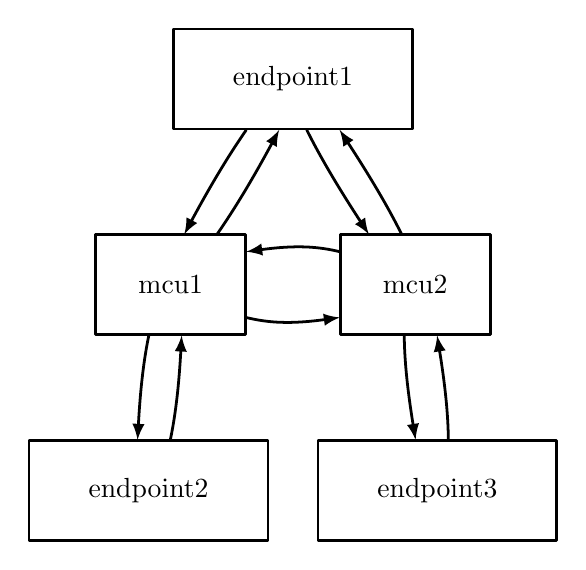
\begin{tikzpicture}[>=latex,line join=bevel,]
  \pgfsetlinewidth{1bp}
%%
\pgfsetcolor{black}
  % Edge: endpoint1 -> mcu2
  \draw [->] (99.961bp,148.71bp) .. controls (104.33bp,139.93bp) and (110.48bp,129.24bp)  .. (122.35bp,111.08bp);
  % Edge: mcu1 -> endpoint2
  \draw [->] (43.107bp,74.708bp) .. controls (41.411bp,66.464bp) and (40.115bp,56.538bp)  .. (39.06bp,37.082bp);
  % Edge: endpoint1 -> mcu1
  \draw [->] (78.208bp,148.71bp) .. controls (72.253bp,140.11bp) and (65.843bp,129.67bp)  .. (55.856bp,111.08bp);
  % Edge: mcu2 -> mcu1
  \draw [->] (111.91bp,104.83bp) .. controls (104bp,106.74bp) and (96.086bp,107.31bp)  .. (78.156bp,104.84bp);
  % Edge: mcu1 -> mcu2
  \draw [->] (78.156bp,81.158bp) .. controls (86.066bp,79.249bp) and (93.976bp,78.684bp)  .. (111.91bp,81.173bp);
  % Edge: endpoint2 -> mcu1
  \draw [->] (50.85bp,37.082bp) .. controls (52.571bp,45.387bp) and (53.885bp,55.431bp)  .. (54.938bp,74.708bp);
  % Edge: mcu2 -> endpoint1
  \draw [->] (134.14bp,111.08bp) .. controls (129.81bp,119.83bp) and (123.66bp,130.52bp)  .. (111.79bp,148.71bp);
  % Edge: mcu1 -> endpoint1
  \draw [->] (67.646bp,111.08bp) .. controls (73.593bp,119.65bp) and (80.009bp,130.08bp)  .. (90.039bp,148.71bp);
  % Edge: mcu2 -> endpoint3
  \draw [->] (135.06bp,74.708bp) .. controls (135.15bp,66.374bp) and (136.02bp,56.322bp)  .. (139.15bp,37.082bp);
  % Edge: endpoint3 -> mcu2
  \draw [->] (150.94bp,37.082bp) .. controls (150.87bp,45.387bp) and (150.01bp,55.431bp)  .. (146.89bp,74.708bp);
  % Node: endpoint1
\begin{scope}
  \definecolor{strokecol}{rgb}{0.0,0.0,0.0};
  \pgfsetstrokecolor{strokecol}
  \draw (52bp,149bp) -- (52bp,185bp) -- (138bp,185bp) -- (138bp,149bp) -- cycle;
  \draw (95bp,167bp) node {endpoint1};
\end{scope}
  % Node: endpoint2
\begin{scope}
  \definecolor{strokecol}{rgb}{0.0,0.0,0.0};
  \pgfsetstrokecolor{strokecol}
  \draw (0bp,1bp) -- (0bp,37bp) -- (86bp,37bp) -- (86bp,1bp) -- cycle;
  \draw (43bp,19bp) node {endpoint2};
\end{scope}
  % Node: endpoint3
\begin{scope}
  \definecolor{strokecol}{rgb}{0.0,0.0,0.0};
  \pgfsetstrokecolor{strokecol}
  \draw (104bp,1bp) -- (104bp,37bp) -- (190bp,37bp) -- (190bp,1bp) -- cycle;
  \draw (147bp,19bp) node {endpoint3};
\end{scope}
  % Node: mcu2
\begin{scope}
  \definecolor{strokecol}{rgb}{0.0,0.0,0.0};
  \pgfsetstrokecolor{strokecol}
  \draw (112bp,75bp) -- (112bp,111bp) -- (166bp,111bp) -- (166bp,75bp) -- cycle;
  \draw (139bp,93bp) node {mcu2};
\end{scope}
  % Node: mcu1
\begin{scope}
  \definecolor{strokecol}{rgb}{0.0,0.0,0.0};
  \pgfsetstrokecolor{strokecol}
  \draw (24bp,75bp) -- (24bp,111bp) -- (78bp,111bp) -- (78bp,75bp) -- cycle;
  \draw (51bp,93bp) node {mcu1};
\end{scope}
%
\end{tikzpicture}

